\chapter{User Interface Structure}
The user interface is implemented in java swing and uses the jchart2d[jchart2d.sourceforge.net] library to display charts and plots. It is divided into two main areas, the control and statistics area (1), whose main purpose is to control the program and display selected statistics, and the data display area (2), which is used to illustrate data via charts and print events in log windows, see figure \ref{fig:ui}. The data display area can contain multiple instances of MetricVisualizers (2.2), MultiScalarVisualizers (2.3) and LogDisplays (2.4).

\begin{figure} [h]
\centering
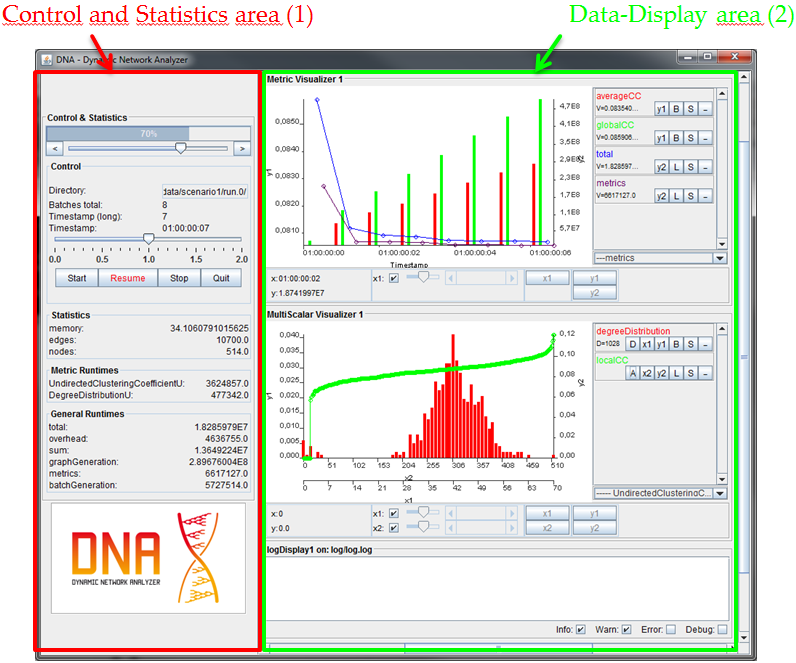
\includegraphics [scale=0.7] {images/ui}
\caption{Example of the two interface areas.}
\label{fig:ui}
\end{figure}

\section{Control and Statistics Area}
The control and statistics area is used to grant general control over the program and to display general statistics and runtimes, see figure \ref{fig:ui2}. It can be divided into two smaller subareas, which will be discussed in the next two chapters. 

\begin{figure} [h]
\centering
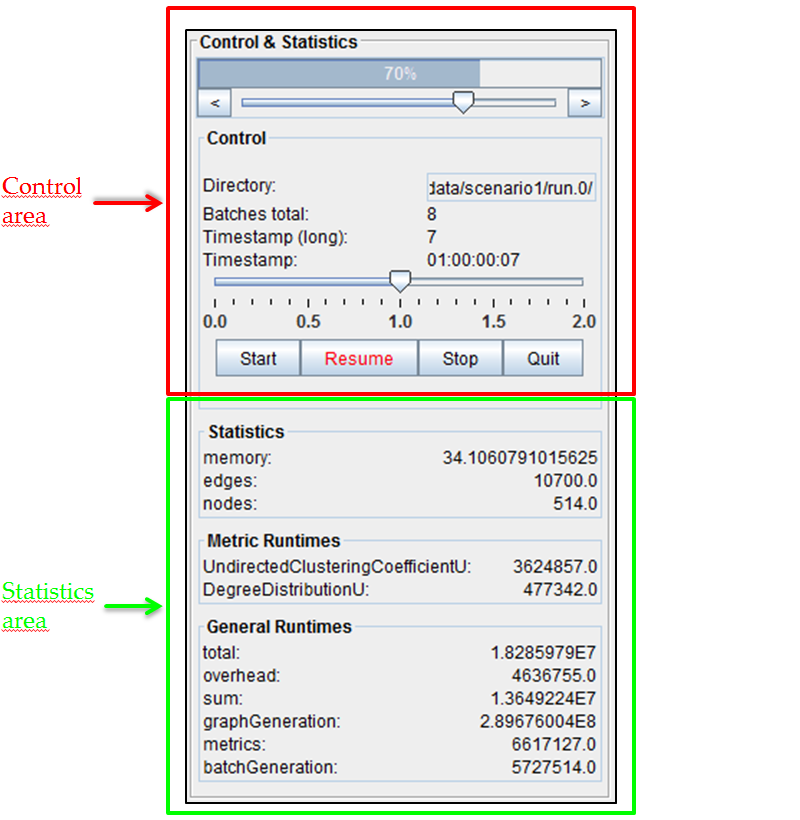
\includegraphics [scale=0.8] {images/ui2}
\caption{Example of the Control and Statistics area during playback mode.}
\label{fig:ui2}
\end{figure}

\subsection{Control Area}
Depending on the used mode, Live-Display or Playback, this area offers different functionalities to control the programs behaviour, see figure \ref{fig:ui3} (a) and (b).

\begin{figure} [h]
\centering
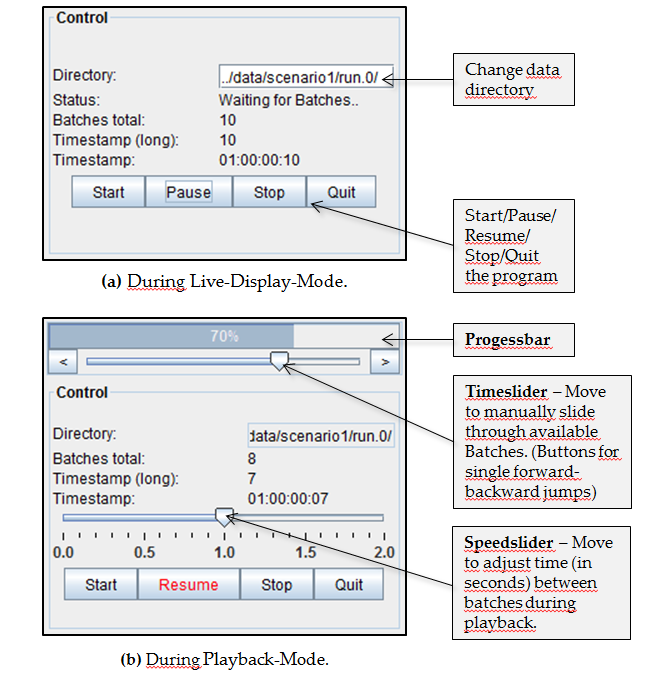
\includegraphics [scale=0.8] {images/ui3}
\caption{Examples of the Control area during different modes.
}
\label{fig:ui3}
\end{figure}

\subsection{Statistics Area}
The statistics area is used to display statistics of the current batch. It can display statistic values aswell as metric and general runtimes. Which values will be displayed can be freely configured. For example, in Figure 2.4 the statistics memory, edges and nodes are being displayed, out of 21 possible values. This is done by defining the desired values in the configuration file and setting the ShowDefinedValues-Flag as true, which will display only the defined values. Setting it to false will result in hiding all defined values and showing all others that are available. See Figure \ref{fig:ui5} on the next page for the configuration code that produced the example in Figure \ref{fig:ui4}.

\begin{figure} [h]
\centering
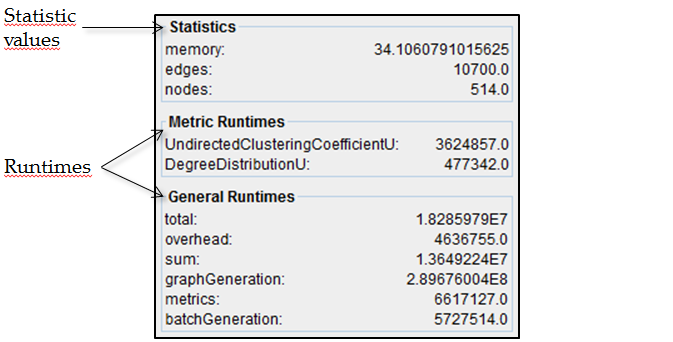
\includegraphics [scale=0.8] {images/ui4}
\caption{Example of a statistics area.}
\label{fig:ui4}
\end{figure}

\begin{figure} [h]
\centering
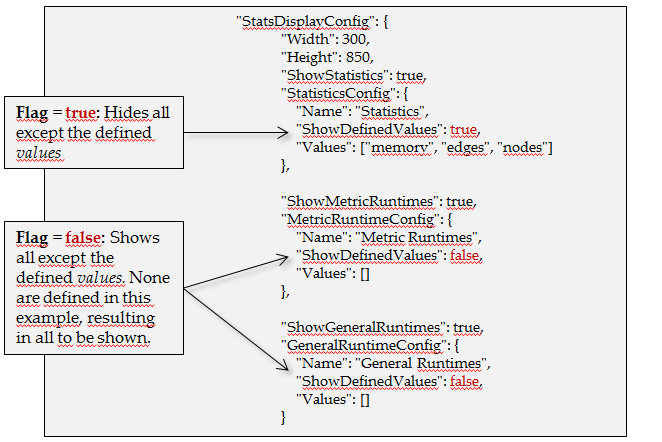
\includegraphics [scale=0.8] {images/ui5}
\caption{Configuration for the Control and Statistics area shown in figure \ref{fig:ui4}.}
\label{fig:ui5}
\end{figure}

\section{Data-Display Area}
The data display area is a flexible part of the interface, which allows the user to monitor the networks properities. It is freely configurable and can contain any amount of Metric Visualizers, MultiScalar Visualizers and LogDisplays,  whose purpose will be discussed in the following chapters. Figure \ref{fig:dataarea} shows an example with one object of each kind.

\begin{figure} [h]
\centering
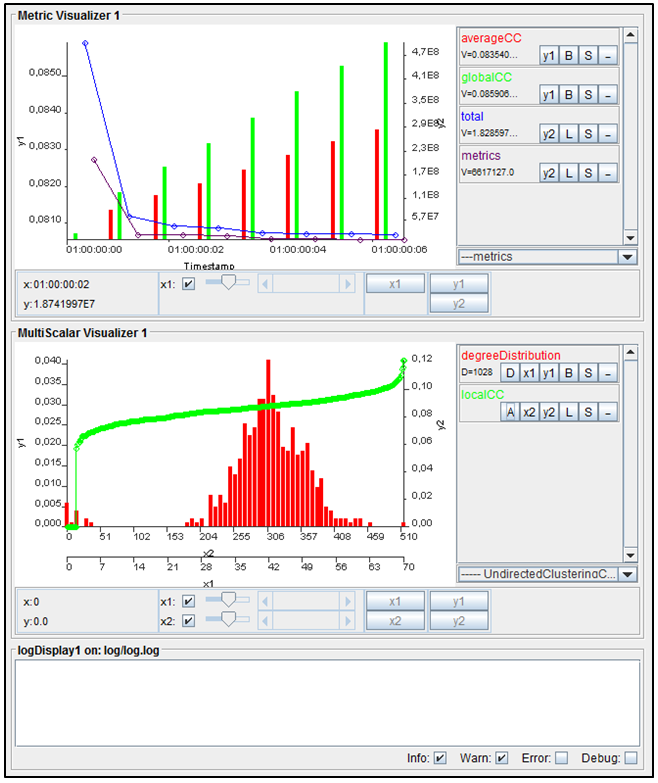
\includegraphics [scale=0.8] {images/dataarea}
\caption{Example of the Data-Display Area.}
\label{fig:dataarea}
\end{figure}

\subsection{Metric Visualizer}
The MetricVisualizer is used to plot metric and statistic data in a chart. All currently shown values are printed in the legend and hold several display features like linespoint-/barplot or switching between y-axis. For example in figure \ref{fig:metricvis1} the value „averageCC“ is plottet as a bar on the y1-axis. New values can be added via the dropdown menu below the legend. The MenuBar allows for additional features for the chart, e.g. show grids for the respective axis or to zoom in on specific intervals of the plot. Which values will be displayed on default can be configured in the configuration file.

\begin{figure} [h]
\centering
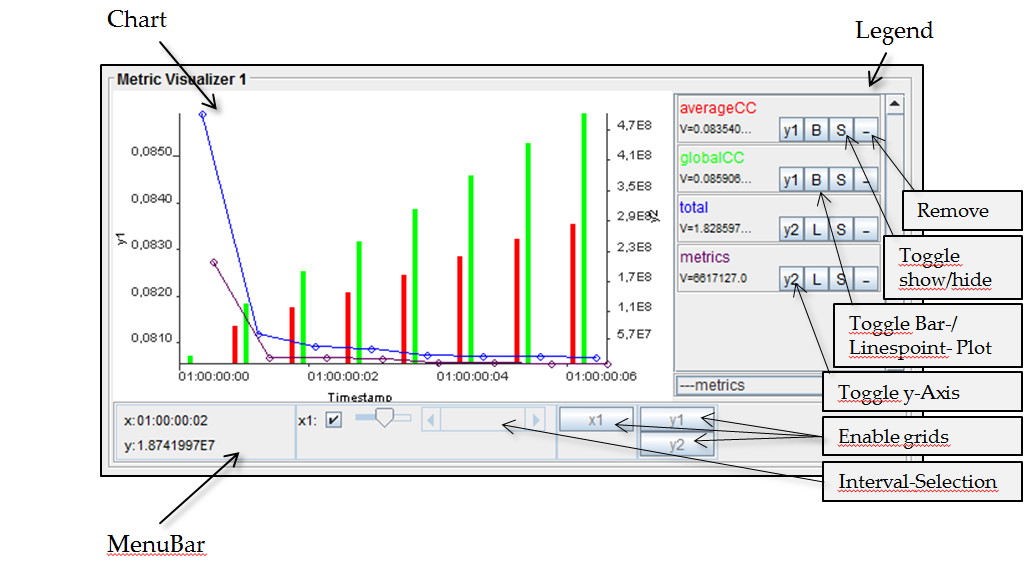
\includegraphics [scale=0.5] {images/metricvis1}
\caption{Example of a MetricVisualizer.}
\label{fig:metricvis1}
\end{figure}

\subsection{MultiScalar Visualizer}
The MultiScalarVisualizer is very similar to the MetricVisualizer. It is used to plot multi scalar values like distributions or nodevaluelists. Additional features are the second x-axis and sorting of the plotted values. For example in figure \ref{fig:multi1}, the nodevaluelist „localCC“ is sorted in ascending order, while the distribution „degreeDistribution“ is plotted as a regular distribution. By clicking on the „D“, it could also be displayed as a CDF.

\begin{figure} [h]
\centering
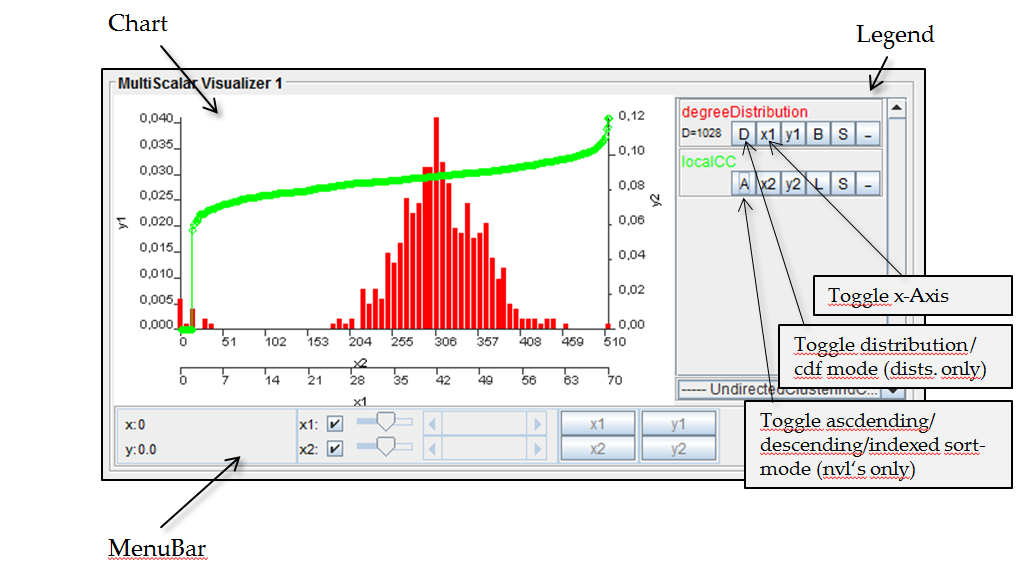
\includegraphics [scale=0.5] {images/multi1}
\caption{Example of a MultiScalar Visualizer}
\label{fig:multi1}
\end{figure}

\subsection{Log Display}
The LogDisplay components are used to tail log files and print relevant informations written to the log. They can filter between four different log-level messages: Info, Warn, Error and Debug, see figure \ref{fig:log}.

\begin{figure} [h]
\centering
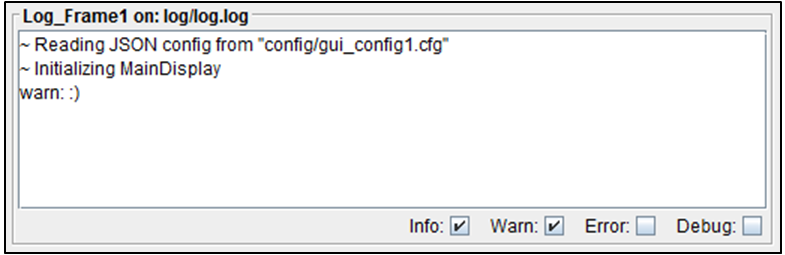
\includegraphics [scale=0.7] {images/log}
\caption{Example of a LogDisplay tailing "log/log.log".}
\label{fig:log}
\end{figure}